\title{A Social Recommender System For Wines}

\iffalse
Page 1: Title Page – including the title of the project, the name of the author, the
date, the word count and the statement specified below under report details.
\fi

\author{
    Undergraduate Project by Peter Chamberlin \\
    BSc Information Systems and Management \\
    Department of Computer Science\\
    Birkbeck, University of London\\
}
\date{\today}

\documentclass[12pt]{article}
% custom paragraph to have line break after using mbox to hack :-/
\newcommand{\myparagraph}[1]{\paragraph{#1}\mbox{}\\}

% import graphicx package so we can import images
\usepackage{graphicx}

% so we can use sidewaystable
% \usepackage[figuresleft]{rotating}

\begin{document}

\maketitle

\iffalse
Page 2: Abstract - One page that summarises the report and the main findings or
results.
\fi

\begin{abstract}
    In this project I implement a recommender system as a web service for wine recommendations. As a starting point the I use the wines, authors and ratings data from wine website Decanter.com, and implement a RESTful web API for accessing wine and author information, augmenting the results with recommendations for other wines or authors.
    The system is written in the Python language, using a MySQL database. The API is built using the Flask framework.
    Implementing a primitive collaborative filtering system but finding my source data to be exceptionally sparse for recommendation, I explore and implement imputation techniques using matrix factorization and singular value decomposition in an attempt to boost the system's ability to make good recommendations.
    I find that both matrix factorization and singular value decomposition improve the recommendation quality of the system, but I am unable to satisfactorily test these systems.
\end{abstract}



\iffalse
Page 3: Table of Contents - including page numbers of each chapter heading and
each appendix.
\fi

\tableofcontents

\iffalse 
Chapter 1: Introduction - the topic, the background, why the topic is relevant or of interest to you, what you hoped to achieve, the aims and objectives of the project.  
\fi

\section{Introduction}

\subsection{Online Recommender Systems}

Since their origin in the mid-1990s with systems such as Tapestry \cite{Goldberg92} and GroupLens \cite{Resnick94}, recommender systems have become ubiquitous on the World Wide Web, being employed by some of the worlds largest online businesses as core parts of their offering.

The growth of the Web has given companies the ability to gather unprecedented amounts of data about their users' preferences, both explicitly collected and inferred from their behaviour, while at the same time enabling them to reach users for less cost more often than ever before.

Amazon's system of product recommendations using item-to-item collaborative filtering is regarded as a ``killer feature''\cite{Fortune12}, and is one of the defining features of the Amazon website. The importance of recommendations to Amazon is reflected in their stated mission, ``to delight our customers by allowing them to serendipitously discover great products''\cite{Fortune12}.

Another company which, like Amazon, is synonymous with recommender systems is Netflix, an ``Internet television network'' \cite{NetflixAbout}. In October 2006 Netflix launched ``The Netflix Prize'', a competition with a \$1,000,000 Grand Prize on offer for any team which could beat their own Cinematch recommender system by ``at least 10\%'' accuracy over a fixed set of data \cite{NetflixPrizeRules}. In 2009 the prize was awarded to the BellKor's Pragmatic Chaos team, who had improved on Netflix's own system by 10.06\% \cite{NetflixPrizeCom}. 

As well as online stores using recommender systems to recommend products a user might be interested in, there are systems \ldots

\subsection{Aims and Objectives}

My interest in recommender systems is founded in their variety and ubiquity. It occurred to me that I encounter, and am the subject of, dozens of these systems in my everyday life. Whether it's Twitter or Facebook recommending interesting interesting people or content to me, Amazon recommending me a book or film, or even a supermarket targeting special offers to me, I interact with recommender systems all the time. I am fascinated both by how these systems work theoretically and by how they are implementated in practice. As such the core objective of my project is to implement a recommender system for a web or mobile application.

I have kindly been permitted to freely use data from Decanter.com's wine reviews database \cite{DecanterWine} for my project. The sphere of wine recommendations is particularly interesting; wine is at first glance a narrow subject, but it is a nuanced one. Among oenophiles there is an emphasis on personal taste and a strong tradition of rating and grading. 

In this project I aim to build a recommender system based on Decanter.com's wine database, identifying and overcoming the challenges associated with the implementation of a real-world recommender system.

The most important aspect of any recommender system may be considered to be the quality of its recommendations, and I intend to focus very strongly on recommendation quality. Nevertheless I do not want to overlook the practical implementation of the system. I aim to produce a system satisfactory in both its recommendations and its performance as a web service, with a robust and elegant implementation in code. 

I will not build any kind of graphical interface for the system, but will instead provide a machine readable API, and where necessary batch scripts and command line tools for preparing and manipulating data.

I aim to satisfy several of the most common use cases for wine recommendation, including user-item, item-item and user-user recommendations.

Overall I hope this project will be a strong learning experience for me\ldots



\iffalse
Chapter 2: Literature Review and Context - the setting of the project in the context of other relevant work or theories or results. How this setting influenced the project.
\fi

\section{Literature Review and Context}\label{literature review}

\subsection{Recommender Systems}

Although the term \textit{recommender system} was not coined until 1997 by Resnick and Varian (Resnick and Varian, 1997 \cite{Resnick97}), the Tapestry system of 1992 (Goldberg et al., 1992 \cite{Goldberg92}) is widely recognised as the first of the kind (Su and Khoshoftaar, 2009 \cite{Su09}). The creators of Tapestry coined the term \textit{collaborative filtering} to describe their method of recommendation, which is based on the principle that if two users rate a number of the same items in a similar manner, then it can be assumed that they will rate other new items similarly (Su and Koshgoftaar, 2009\cite{Su09}).

Su and Khoshgoftaar (2009 \cite{Su09}) point out that although collaborative filtering has been widely adopted as a general term to describe systems making recommendations, many such systems do not explicitly collaborate with users or exclusively filter items for recommendation. In fact the term recommender system itself was coined by Resnick and Varian in response to the inadequacy of collaborative filtering for describing the plurality of techniques that were beginning to become associated with it. Recommender system is intentionally a broader term, describing any system that ``assists and augments [the] natural social process'' of recommendation (Resnick and Varian, 1997 \cite{Resnick97}).

In his 2002 survey of the state of the art in recommender systems, Robin Burke presents five categories of recommender (Burke, 2002 \cite{Burke02}). I have reproduced his table of recommendation techniques in Table \ref{table:burke02}. Burke presents five main categories of filtering technique: collaborative, \textit{content-based}, \textit{demographic}, \textit{utility-based} and \textit{knowledge-based} (Burke, 2002 \cite{Burke02}).

\begin{table}[ht]
    \caption{Recommendation Techniques, reproduced from Burke, 2002 \cite{Burke02}}
    \centering
    \begin{tabular}{p{2.5cm} p{3.5cm} p{3.5cm} p{3.5cm}}
        Technique & Backgroud & Input & Process
        \\\hline\hline
        Collaborative & Ratings from \textit{U} of items in \textit{I}. & Ratings from \textit{u} of items in \textit{I}. & Identify users in \textit{U} similar to \textit{u}, and extrapolate from their ratings of \textit{i}. \\
        Content-based & Features of items in \textit{I}. & \textit{u}'s ratings of items in \textit{I}. & Generate a classifier that fits \textit{u}'s rating behaviour and use it on \textit{i}. \\ 
        Demographic & Demographic information about \textit{U} and their ratings of items in \textit{I}. & Demographic information about \textit{u}. & Identify users that are demographically similar to \textit{u}, and extrapolate from their ratings of \textit{i}. \\
        Utility-based & Features of items in \textit{I}. & A utility function over items in \textit{I} that describes \textit{u}'s preferences. & Apply the function to the items and determine \textit{i}'s rank. \\
        Knowledge-based & Features of items in \textit{I}. Knowledge of how these items meet a user's needs. & A description of \textit{u}'s needs or interests. & Infer a match between \textit{i} and \textit{u}'s need. \\
        \\\hline
    \end{tabular}
    \label{table:burke02}
\end{table}

These five kinds of system are classified using three properties: \textit{background data}, \textit{input data} and \textit{process} (Burke, 2002 \cite{Burke02}). Background data is that which exists before and independant of the recommendation, such as previous stated preferences of a group of users \textit{U} for a set of items \textit{I}. Input data is that which is considered by the system when making recommendations, such as the ratings of an individual \textit{u} of items in \textit{I}. Process is the method by which recommendations are arrived at by application of the input data and the background data (Burke, 2002 \cite{Burke02}). These three aspects provide a good lens through which to compare the different approaches.

\subsubsection{Collaborative Filtering}

Collaborative filtering is ``the technique of using peer opinions to predict the interest of others'' (Claypool et al., 1999 \cite{Claypool99}), and uses the ratings of a set of users \textit{U} over a set of items \textit{I} as background data, and the ratings of each individual user \textit{u} of items in \textit{I} as input data. The process of recommendation is to identify similar users to \textit{u} in \textit{U}, and then to infer their preferences for items in \textit{I} based on the preferences of those similar users (Burke, 2002 \cite{Burke02}).

In 2002 Burke described collaborative filtering as the most widely used and mature of these types (Burke, 2002 \cite{Burke02}), citing GroupLens (Resnick, 1994 \cite{Resnick94}) and Tapestry (Goldberg, 1992 \cite{Goldberg92}) as important examples of such systems. From my observations of more recent literature that remains the case. Collaborative filtering is still certainly among the most widely used of these techniques, with Su and Khoshgoftaar describing a large number of collaborative filtering-based systems in their 2009 survey (Su and Koshgoftaar, 2009 \cite{Su09}).

Even in its most basic form there are many potential methods for measuring similarity between users in a collaborative filtering system. The most simple are such distance metrics such as Manhattan distance or Euclidean distance (Segaran, 2007 Ch.2 \cite{Segaran07}). One of the most commonly used and relatively simple measures of similarity is the Pearson correlation coefficient, which is even used in quite advanced systems (Segaran, 2007 Ch.2 \cite{Segaran07}).

There are a number of issues associated with the application of pure collaborative filtering, however, which hamper its application in many instances:

\begin{itemize}
    \item Early rater problem, whereby an item entering the system with no ratings has no chance of being recommended (Claypool et al., 1999 \cite{Claypool99}).
    \item Sparsity problem. Where there is a high ratio of items to ratings it may be difficult to find items which have been rated by enough users to use as the basis for recommendation (Claypool et al., 1999 \cite{Claypool99})(Su and Koshgoftaar, 2009 \cite{Su09}).
    \item Grey sheep, which are users who neither conform nor disagree with any other group in a significant way, making it very difficult to recommend items for them (Claypool et al., 1999 \cite{Claypool99})(Su and Koshgoftaar, 2009 \cite{Su09}).
    \item Synonymy, whereby identical items have different names or entries. In this case the collaborative filtering systems are unable to detect that they are the same item (Su and Koshgoftaar, 2009 \cite{Su09}).
    \item Vulnerability to shilling, where a user may submit a very large number of ratings to manipulate the recommendation of items (Su and Koshgoftaar, 2009 \cite{Su09}).
\end{itemize}

Much of the variation between collaborative filtering techniques described by Su and Khoshgoftaar (2009 \cite{Su09}) can be attributed to efforts by system developers to minimise the impact of one or more of these problems by introducing auxiliary methods.

\subsubsection{Content-based}

In content-based filtering systems the features of items in \textit{I} form the background data, and the user \textit{u}'s ratings serve as the input data. The process of recommendation depends on building a classifier that can predict \textit{u}'s rating behaviour in respect of an item \textit{i} based on \textit{u}'s previous ratings of items in \textit{I} (Burke, 2002 \cite{Burke02}).

Content-based, like collaborative filtering, builds up a long term profile of a user's interests and preferences (Burke, 2002 \cite{Burke02}). Researchers have developed systems which successfully combined content-based and collaborative filtering systems to produce better recommendations. Claypool et al. describe such a system which predicts ratings based on a weighted average of results from each system, with the weighting varying per user in order to achieve optimal results (Claypool et al., 1999 \cite{Claypool99}).

\subsubsection{Demographic}

Demographic recommender systems use demographic information about users \textit{U} and their ratings in \textit{I} as background data, with demographic information about \textit{u} as the input data. The recommendation process depends on matching \textit{u} with other demographically similar users in \textit{U} (Burke, 2002 \cite{Burke02}).

\subsubsection{Utility-based}

Utility-based systems use features of items in \textit{I} as their background data, and depend on a utility function representing \textit{u}'s preferences in order to arrive at recommendations. The process is the application of the function for \textit{u} to the items \textit{I} (Burke, 2002 \cite{Burke02}).

\subsubsection{Knowledge-based}

Knowledge-based systems, like utility-based systems, draw on the features of items in \textit{I} as their background data. As input data they require information about \textit{u}'s needs. The process is to infer a need for one or more items in \textit{I} (Burke, 2002 \cite{Burke02}).

Knowledge-based systems can also benefit from being combined with collaborative filtering systems, in a way that may improve an under-performing knowledge-based system, but without realising pure collaborative filtering's ability to identify niche groups (Burke, 1999 \cite{Burke99b}).

\subsection{Recommending Wines.}

Recommender systems for wines are not a new idea, being typical of the kind of item many systems are designed to recommend. Burke developed the VintageExchange FindMe recommender system in 1999 (Burke, 1999 \cite{Burke99}), and there is at least one patent pending with the WIPO for a wine recommender system as an aid to salespeople or waiting staff (Ward et al., 2012 \cite{WIPO12}).

Burke's FindMe, a knowledge-based recommender system, ``required approximately one person-month of knowledge engineering effort'' (Burke, 1999b \cite{Burke99b}) in order to perform well. Such knowledge-based systems are required to recognise the importance of given product features, and so require a great deal of priming (Burke, 1999b \cite{Burke99b}).

Another wine recommender system is the Tetherless World Wine Agent (TWWA) (Patton, 2010 \cite{Patton10}). The TWWA project is primarily concerned with knowledge representaion and the Semantic Web, presenting a common and collaborative ontology for wine with which users can share wine recommendations across their social networks (TWWA, 2013 \cite{TWWAIndex}). The system does not automatically tailor recommendations to users, although this is stated as a target for future work (TWWA, 2013 \cite{TWWAIndex}).

\subsection{Evaluating Recommender Systems}

Shani and Gunawardana (2011 \cite{Shani11}) describe several approaches to the evaluation of recommender systems, including different experimental settings and a number of different statistical methods. They highlight the different aspects of recommender systems that can be evaluated, including prediction accuracy; how accurately does the system predict ratings or preferences, item-space coverage; what proportion of the items in the system are recommendable, and user-space coverage; the proportion of users or interactions the system can provide recommendations for (Shani and Gunawardana, 2011 \cite{Shani11}).

In terms of prediction accuracy mean absolute error (MAE), and root mean squared error (RMSE) are the most popular measures (Shani and Gunawardana, 2011 \cite{Shani11}), which Su and Khoshgoftaar (2009 \cite{Su09}) call ``predictive accuracy metrics''. 

There is some criticism of accuract metrics applied to recommender systems. McNee, Riedl and Konstan (2006 \cite{McNee06}) cite Amazon.com as a case in point, where on the page for a book by a given author you will find recommendations for other of the same author's books. They argue that this is not interesting for the user, and that there is a need for recommender systems developers to look beyond simply the ratability of systems, concluding, ``It is now time to also study recommenders from a user-centric perspective to make them not only accurate and helpful, but also a pleasure to use'' (McNee et al., 2006 \cite{McNee06}).

\subsection{Web Services and Service Oriented Architecture}

Service oriented architecture (SOA) is an increasingly widely used paradigm in enterprise applications, enabling such benefits as modularity, distribution and reuse of services (Sheikh et al., 2011 \cite{Sheikh11}). SOA systems are loosely coupled, and lend themselves to supporting heterogeneous applications (Benatallah and Nezhad, 2008 \cite{Benatallah08}), such as would be the case for a service providing data for a variety of websites or mobile applications. Web SOAs encompass traditional WS-* web services approaches, such as SOAP and XML, as well as the more recently emerging RESTful (REpresentational State Transfer) approach, which takes advantage of the existing communications protocol of HTTP, and associated protocols such as SSL (Benatallah and Nezhad, 2008 \cite{Benatallah08}). RESTful and WS-* have their benefits and weaknesses, and the choice of either would be dependant on the needs of any given service. 

Pautasso et al. (2008 \cite{Pautasso08}) critically compare WS-* and RESTful services, concluding that although REST is limited by the contraints of the HTTP protocol, its restictive nature and architecture are also a strength, ``choosing REST removes the need for making a series of further architectural decisions related to the various layers of the WS-* stack and makes such complexity appear as superfluous'' (Pautasso et al., 2008 \cite{Pautasso08}).

\subsection{Implications}

There is extensive literature on recommender systems, so much so that it is very difficult to assess the pros and cons of any given approach in respect of my project. One theme that is very strong in recommender systems is that of collaborative filtering, which is central to the majority of systems I have looked at. In many cases collaborative filtering is used in conjunction with other methods that boost or tune the results. For that reason I intend to pursue collaborative filtering in my system, and will incorporate strategies to improve recommendations iteratively.

With regard to the web application component of my system, it seems clear that a RESTful web service would be suitable. My system will have a small number of API endpoints, so I will be able to reap the benefits the simplicity of the RESTful web stack without suffering the difficulties associated with its limited customisability.



\section{Method}\label{method}

\iffalse
the overall approach and rationale.
Why the project was tackled in the chosen way, and why other ways were ruled out.
\fi

\subsection{Methodology}

Given the exploratory nature of this project I elected to take an incremental and iterative approach, developing small parts of the system at any time (increments), and iterating over those parts with improvements as necessity dicated and time allowed. This approach is based on that laid out by Cockburn (2008 \cite{Cockburn08}).

\subsubsection{Phases}

The main phases of development would be:

\begin{enumerate}
    \item Clean up and migrate data
    \item Create initial API app
    \item Connect API with database
    \item Implement routes for API access to wines and authors
    \item Augment API routes for wines and authors with recommendations
    \item Iterate on recommendation methods, evaluating and improving quality
\end{enumerate}

My reason for taking this approach, rather than following a formal development methodology such as the waterfall model, was that my aims and objectives were unbounded, it the sense that there would not be a point at which my system was complete, only a point at which it was minimally complete, followed by a succession of points at which is was improved.

\subsubsection{Minimum Viable Product}

It was clear that I would be doing a large amount of experimental programming, and given my lack of prior experience in the problem domain I felt it inappropriate to attempt to quantify my expectations for the system in terms of detailed requirements. Nevertheless there were very clear minimum objectives for the system, without which it would not be possible to claim any degree of success.

The system should at least:

\begin{itemize}
    \item Provide an HTTP API for accessing wine and user information from the Decanter.com tastings database.
    \item Augment the API results for wines and authors with appropriate recommendations of other similar or interesting wines and author.
    \item Provide API results suitable for machine interpretation by web or mobile applications.
    \item Provide a mechanism by which to evaluate recommendation quality.
\end{itemize}

These requirements in the least should be fulfilled by the system. With this having been done the focus of the project will be on maximising the quality of recommendations.

\subsection{Technologies and Tools}

\subsubsection{Python}

As the main progamming language for my project I chose to use Python. There were several candidate languages, not least Java, but I decided on Python because it has a number of attributes which lent themselves particularly to this project:

\begin{itemize}
    \item Extensive mathematical and scientific libraries, such as numpy \cite{Numpy} and scipy \cite{Scipy}.
    \item Extensive detailed documentation \cite{PythonDocs}.
    \item Widely used in web development, such as by Google and YouTube \cite{PythonQuotes}.
    \item Interactive interpreter, allowing command line interaction and supporting scripting on Unix-like systems \cite{PythonInterpreter}.
\end{itemize}

One deciding factor was that my first enquiry into recommender systems was reading Segaran's code examples in Chapter 2 of Collective Intelligence (2007, Ch.2 \cite{Segaran07}), where the language he uses for his code examples is Python. 

In addition to its suitability for tasks around recommender systems, Python has a solid heritage of web application frameworks, such as Django \cite{DjangoProject} and Flask \cite{Flask}. Django is a fully featured website building framework, and as such carries many features unnecessary for my project, whereas Flask, a ``micro-framework'' \cite{Flask}, appeared to be more lightweight and simple to implement. Therefore I chose to implement my API using Flask \cite{Flask}.

For the most part I considered that my system would suit the stateless, non-persistent nature of a Python web application. The only concern in this regard would be that I would need to recreate objects in memory from scratch with each request rather than persist them as I might using another language, such as using Java with the JPA\cite{JavaJPA}. It was reasonable to suppose that in generating recommendations I would potentially be creating large objects in memory, and that there may be a performance deficit incurred by having to rebuild such object on a per request basis. I resolved that should the lack of persistence prove problematic down the line I would be able to use a persistence mechanism such as Memcached \cite{PythonMemcached} to serve this purpose, and found that there is wide support for such a solution using Python and Flask \cite{FlaskMemcached}.

\subsubsection{MySQL}

Originally I had envisaged a system backed by a PostgreSQL \cite{PostgreSQL} RDBMS, but having received the Decanter.com data as a MySQL \cite{MySQL} database it did not seem, comparing the two systems, that there would be any significant benefit migrating the data to PostgreSQL. Both are widely used in production, and have similar feature sets. For a short time I considered using a NoSQL database such as MongoDB \cite{MongoDB} for my project, but decided against such a solution, recognising that such document-oriented systems are not ideal when joining between tables in the way that I would need to for my wines and tasting notes. It seemed that an RDBMS was ideally suited to the purpose, and there was no reason why that shouldn't be MySQL.

\subsubsection{GitHub}

Given the iterative nature of my development process I envisaged a need to be able to easily version my source code, possibly running several different versions at once, with the ability to revert changes back to any previous state. I also wanted a remote backup of my system in case of problems with my own development computer. In order to do be able to do these things I chose to store my code as a project in GitHub \cite{GitHub}, which is a web service providing Git version control. I chose to use GitHub for my notes and project files also, so that my entire project was stored, versioned and backed up together.



\section{The Sommelier System}\label{design}

\myparagraph{Data Cleanup}

The data source I have used for my project is the wines database belonging to Decanter.com\cite{DecanterCom}. The database contains nearly 40,000 professional ratings and tasting notes for wines from as far back as 1986, featuring vintages as far back as 1917.

The original database is highly inconsistent, displaying a mixture of design approaches and a variable quality of data. This is consistent with the fact that the database has been developed over a long period of time by a number of different developers with varying levels of skill, and that wine journalists making entries into the database have taken a number of idiosyncratic approaches to data entry.

Nevertheless I considered there to be a great deal of useful and interesting information in the database, with it to contain usable ratings and/or tastings for over 33,000 wines.

\begin{figure}[h!]
    \caption{Decanter.com Database}
    \centering
        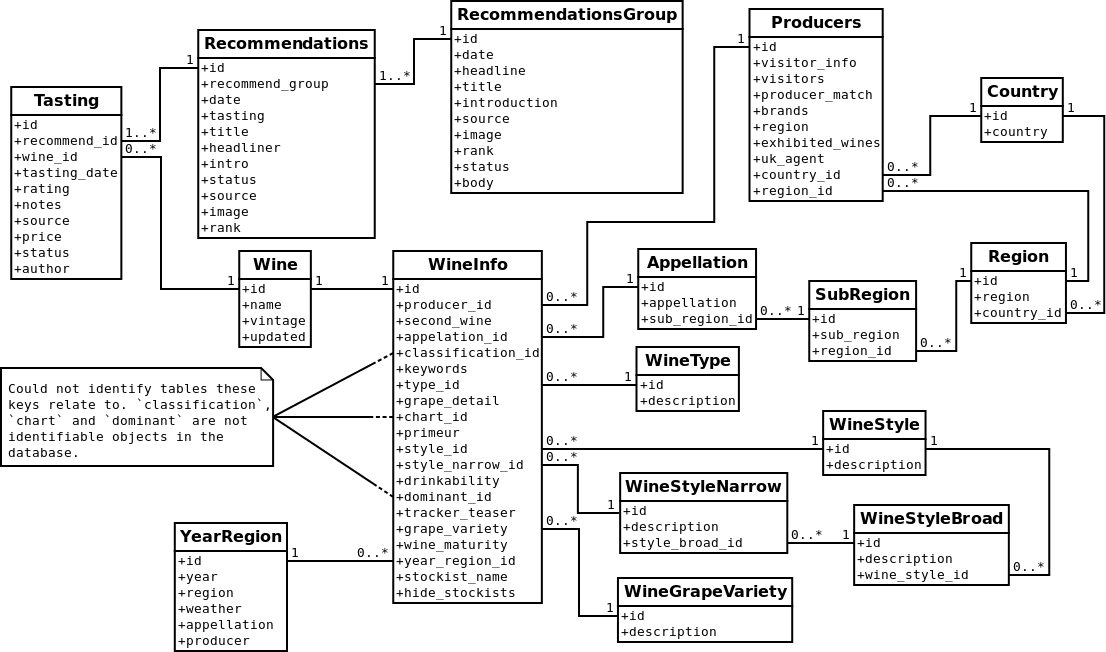
\includegraphics[width=14cm]{DecanterWineDB}
    \label{fig:decanterdb}
\end{figure}

The WineInfo table is a mixture of foreign keys joining to very small tables, such as WineInfo.type\_id joining to WineType.id where WineType is a table with only two attributes. This approach, stiving for a high degree of normalisation, contrasts with the fact that the same table also has the attribute second\_wine, as a string which only holds data in 450 of the 38762 entries in the table.

\myparagraph{Creating The Sommelier Dataset}

\begin{figure}[h!]
    \caption{Sommelier Database}
    \centering
        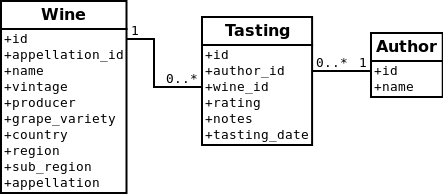
\includegraphics[width=10cm]{SommelierDBSimple}
    \label{fig:sommelierdb}
\end{figure}

For the new Sommelier database, Figure \ref{fig:sommelierdb}, I decided to denormalise [explanation/citation needed!] the wine data. This enables the data to be queried without joins, maximising the simplicity and execution speed of the queries [citation needed]. Denormalization makes data integrity difficult to maintain however, as there are potentially a large number of records to update for any change in a duplicated value. In this case an appellation or sub-region name changing might require thousands of records to be amended. Creating and editing wines is not a requirement of my system though, so for the purposes of this project the wine and tasting data is static and will not be subject to updates. For this reason the duplication of data within the Wine records is not problematic. In a real world setting this would need to be revisited.

Much of the data from the original database was disregarded entirely.

The tables WineStyleNarrow and WineStyleBroad contained generic text descriptions for wine (``rich and creamy'', ``crisp and tangy'' etc.). I initially considered this to have potential for migration into tag data which I could reuse as part of my filtering. Unfortunately less than 6435 of the records in WineInfo had non-null values for their style\_narrow\_id field, and only 3397 of these had corresponding records in the Tasting table. This figure was only around 10\% of the number of wines I expected the Sommelier database to contain so I decided that the WineStyle* tables were probably not worthwhile to migrate.

The WineType table was ignored because no wines corresponded to it; no WineInfo.type\_id record matched any WineType.id.

\myparagraph{The Author Problem}

The biggest shortcoming of the dataset is that the author of a tasting note is often not recorded. The number of wines with notes and known authors is only 1401, with there being 18 named authors on the system. 

Table \ref{table:authors} shows the distribution of tastings amongst authors, only 5 of which have tasted and rated more than 100 wines in the database.

\begin{table}[ht]
\caption{Authors of tasting notes and ratings}
\centering
\begin{tabular}{c c}
\\\hline\hline
Author               & Wines tasted, with notes and rating
\\\hline
Amy Wislocki         &            28 \\
Andrew Jefford       &           105 \\
Beverley Blanning MW &            13 \\
Carolyn Holmes       &             1 \\
Christelle Guibert   &           119 \\
Clive Coates MW      &             6 \\
David Peppercorn     &            44 \\
Gerald D Boyd        &             7 \\
Harriet Waugh        &           250 \\
James Lawther MW     &           226 \\
John Radford         &             2 \\
Josephine Butchart   &            24 \\
Norm Roby            &             4 \\
Rosemary George MW   &             6 \\
Serena Sutcliffe     &            31 \\
Stephen Brook        &            19 \\
Steven Spurrier      &           497 \\
\\\hline
\end{tabular}
\label{table:authors}
\end{table}

In some cases an author's initials or full name are recorded within the text of a tasting note. I decided that extracting and making use of these was impractical given the time constraints of this project.

DESCRIBE DATA SETS BEFORE AND AFTER

THE SOMMELIER DATASET

Having analysed the dataset and conceived an ideal schema, I needed to decide what the criteria to apply when extracting my new dataset from the source data.

Given that the purpose of the dataset is social recommendations, the first decision I made was to discard any wines without both tasting notes and a rating, whether.


\section{Testing and Evaluation}\label{testing}
How well does the system work? Details of testing and evaluation of the system\ldots




\section{Conclusion}\label{conclusions}
Was the project successful?




\section{Review}\label{review}
Review / reflections of the project on a personal level. What has been achieved? What were the problems, and how were they overcome?




\begin{thebibliography}{9}

    \bibitem{Burke99} Burke, R., \emph{The Wasabi Personal Shopper: A Case-Based Recommender System}, 1999. Submitted to the 11th Annual Conference on Innovative Applications of Artificial Intelligence.

    \bibitem{Burke99b} Burke, R., \emph{Integrating Knowledge-Based and Collaborative-Filtering Recommender Systems}, 1999. In: Artificial Intelligence for Electronic Commerce: Papers from the AAAI Workshop (AAAI Technical Report WS-99-0 1), pp.69-72.

    \bibitem{Burke00} Burke, R., \emph{Knowledge-Based Recommender Systems}, Encyclopedia of Library and Information Systems, 2000. Marcel Dekker.

    \bibitem{Burke02} Burke, R., \emph{Hybrid Recommender Systems: Survey and Experiments}, User Modeling and User-Adapted Interaction, Volume 12 Issue 4, November 2002, Pages 331 - 370. Kluwer Academic Publishers: Hingham, MA, USA

    \bibitem{Debnath08} Debnath, Souvik and Ganguly, Niloy and Mitra, Pabitra, \emph{
        Feature weighting in content based recommendation system using social network analysis}, Proceedings of the 17th international conference on World Wide Web, WWW '08, 2008, Beijing, China, Pages 1041 - 1042. ACM: New York, NY, USA,

    \bibitem{Goldberg92} Goldberg, D. Nichols, D., Oki, B. M., and Terry, D., \emph{Using collaborative filtering to weave an information tapestry}, Commun. ACM 35, 12 (Dec. 1992), 61--70.

    \bibitem{Fortune12} Mangalindan, J. P., \emph{Amazon's Recommendation Secret}, July 2012. URL: http://tech.fortune.cnn.com/2012/07/30/amazon-5/

    \bibitem{Patton10} Patton, E., McGuinness, D., \emph{Scaling the Wall: Experiences Adapting a Semantic Web Application to Utilize Social Networks on Mobile Devices}, 2010. In: Proceedings of the WebSci10: Extending the Frontiers of Society On-Line, April 26-27th, 2010, Raleigh, NC: US.

    \bibitem{Resnick94} Resnick, P., Iacovou, N., Sushak, M., Bergstrom, P., Riedl, J., \emph{GroupLens: An open architecture for collaborative filtering of netnews}, 1994 ACM Conference on Computer Supported Collaborative Work, 1994. Association of Computing Machinery, Chapel Hill, NC.

    \bibitem{Resnick97} Resnick, P., Varian, H. R., \emph{Recommender Systems}, 1997. Communications of the ACM, 40 (3), 56-58. Association of Computing Machinery, Chapel Hill, NC.

    \bibitem{TWWAIndex} http://wineagent.tw.rpi.edu/index.php

\iffalse
A. Y. Ng and M. I. Jordan. On discriminative vs generative
classifiers: A comparison of logistic regression and naive
bayes. In Neural Information Processing Systems, pages
841–848, Vancouver, Canada, december 2001. MIT Press.
2
Robles, V.; Larranaga, P.; Menasalvas, E.; Perez, M.S.; Herves, V.; , "Improvement of naive Bayes collaborative filtering using interval estimation," Web Intelligence, 2003. WI 2003. Proceedings. IEEE/WIC International Conference on , vol., no., pp. 168- 174, 13-17 Oct. 2003
doi: 10.1109/WI.2003.1241189
keywords: {Algorithm design and analysis;Clustering algorithms;Collaboration;Collaborative work;Data mining;Filtering algorithms;Probability;Recommender systems;Scalability;Training data; Bayes methods; Web sites; groupware; information filters; learning (artificial intelligence); statistical analysis; Bayesian classifier; UCl repository; Web data; collaborative filtering; ecommerce site; interval estimation; naive Bayes method; recommender system; semi naive Bayes method;}
URL: http://ieeexplore.ieee.org/stamp/stamp.jsp?tp=&arnumber=1241189&isnumber=27823

Xiaoyuan Su; Greiner, R.; Khoshgoftaar, T.M.; Xingquan Zhu; , "Hybrid Collaborative Filtering Algorithms Using a Mixture of Experts," Web Intelligence, IEEE/WIC/ACM International Conference on , vol., no., pp.645-649, 2-5 Nov. 2007
doi: 10.1109/WI.2007.10
keywords: {Clustering algorithms;Collaborative work;Computer science;Filtering algorithms;International collaboration;Motion pictures;Niobium;Predictive models;Recommender systems;USA Councils;information filtering;content-boosted CF;experts mixture;hybrid collaborative filtering algorithms;memory-based algorithms;pure content-based CF algorithms;pure model-based algorithms;sequential mixture CF;}
URL: http://ieeexplore.ieee.org/stamp/stamp.jsp?tp=&arnumber=4427165&isnumber=4427044

Xiaoyuan Su; Taghi M. Khoshgoftaar; , "Collaborative Filtering for Multi-class Data Using Belief Nets Algorithms," Tools with Artificial Intelligence, 2006. ICTAI '06. 18th IEEE International Conference on , vol., no., pp.497-504, Nov. 2006
doi: 10.1109/ICTAI.2006.41
keywords: {Bayesian methods;Collaboration;Collaborative work;Filtering algorithms;Logistics;Predictive models;Recommender systems;Regression tree analysis;Robustness;Scalability;belief networks;data handling;groupware;information filtering;Bayesian belief nets;Pearson correlation-based collaborative filtering;data sparseness;extended logistic regression;multiclass collaborative filtering data;recommender system;tree augmented naive Bayes model;}
URL: http://ieeexplore.ieee.org/stamp/stamp.jsp?tp=&arnumber=4031936&isnumber=4031859



BibTex:

@INPROCEEDINGS{Burke00knowledge-basedrecommender,
author = {Robin Burke},
title = {Knowledge-Based Recommender Systems},
booktitle = {ENCYCLOPEDIA OF LIBRARY AND INFORMATION SYSTEMS},
year = {2000},
pages = {2000},
publisher = {Marcel Dekker}
}

@conference {236,
title = {GroupLens: An open architecture for collaborative filtering of netnews},
booktitle = {1994 ACM Conference on Computer Supported Collaborative Work Conference},
year = {1994},
month = {10/1994},
pages = {175-186},
publisher = {Association of Computing Machinery},
organization = {Association of Computing Machinery},
address = {Chapel Hill, NC},
abstract = {<p class=``abstract''>Collaborative filters help people make choices based on the opinions of other people. GroupLens is a system for collaborative filtering of netnews, to help people find articles they will like in the huge stream of available articles. News reader clients display predicted scores and make it easy for users to rate articles after they read them. Rating servers, called Better Bit Bureaus, gather and disseminate the ratings. The rating servers predict scores based on the heuristic that people who agreed in the past will probably agree again. Users can protect their privacy by entering ratings under pseudonyms, without reducing the effectiveness of the score prediction. The entire architecture is open: alternative software for news clients and Better Bit Bureaus can be developed independently and can interoperate with the components we have developed.</p>},
doi = {http://doi.acm.org/10.1145/192844.192905},
author = {Resnick, P. and Iacovou, N. and Sushak, M. and Bergstrom, P. and J. Riedl}
}


\fi

\end{thebibliography}



\end{document}
Chapter 3: Research/Development Method - the overall approach and rationale.
Why the project was tackled in the chosen way, and why other ways were ruled out.
Chapter 4: Data/Findings/Designs - the project outcome. This might be data
collected and tabulated or the design of a program, or whatever outcome was
obtained.
Chapter 5: Analysis/Evaluation/Testing – assessing or testing the project outcome.
If the project is of type 2 are the results plausible? If the project is of type 3 or 4 then
any computer code should be tested using a range of inputs.
Chapter 6: Conclusions/Recommendations - as a result of the project. The project
does not need to have a positive conclusion. For example, it might prove that some
system was not effective or successful. You should indicate to what extent your
objectives have been achieved.
Chapter 7: Review/Reflections - this is often missed out by students but is very
important. It is an opportunity to, firstly, review on a personal level what you have
achieved, how you achieved it, what took the most time, the problems faced, the way
in which they were overcome, etc. Secondly, it is an opportunity to reflect on the
project with the benefit of hindsight. What might have been done differently? Was the
research method adequate? How could the project have been more successful?
Examiners like to see evidence of learning and mature reflection
Chapter 8: References - all references should be cited in the body of the report. A
typical reference in the report might take the form, “Donar and Kebab (1996) suggest
that high cholesterol levels do not lead to heart disease\ldots.” or “empirical eating studies
show that\ldots. (Donar and Kebab, 1996)”. The full title of the article or book or web
page in which Donar and Kebab make these assertions is then given in the list of
references. Where possible, use an article or a book rather than a web page. The idea
of references is not just to substantiate statements and arguments but also to make it
possible for other people to find the references. Normally, for a book, you should list
author(s), title, publisher, date of publication, relevant page number(s). It can be
difficult to locate the relevant part of a book if the page numbers are omitted. For an
article list author(s), title of article, name of journal, volume and issue number, date,
and page numbers of the article. In the academic world references are regarded as
very important and poor referencing will certainly detract from the project report. Do
not under any circumstances quote from a source without making it clear that
you are quoting. Any quote must be accompanied by an appropriate reference.
Chapter 9: Bibliography - list any relevant literature that has not been cited in the
report. (It is not a very well-kept secret that examiners tend to think that anything in a
bibliography has not in fact been read by the student. Of course this is a monstrous
slur but nevertheless do not waste too much time on the bibliography. Concentrate on
the references!)
Chapter 10: Appendices - these are not obligatory. Only put in relevant items not
already in the body of the report. These might include a questionnaire used to gather
information, a list of the people interviewed and their companies, transcripts of
interviews, detailed data, program listings, test results, etc. Any appendix should be
referred to in the main part of the report and not just stuck at the end of the report
without explanation. It is very important that an examiner can find evidence for the
claims you make in your report. The appendices are the place to put such evidence
without cluttering up the main part of the report.

